\chapter{Analisis}
\label{chap:analisis}
\section{Analisis konversi menuju \textit{CodeIgniter 4}}
Konversi \textit{CodeIgniter 3} menuju \textit{CodeIgniter 4} diperlukan penulisan ulang karena terdapat perubahan struktur aplikasi dan beberapa fungsi yang memiliki pemanggilan berbeda dan harus dilakukan pembaharuan.
\subsection{Persiapan \textit{CodeIgniter 4}} Konversi dimulai dengan mempersiapkan aplikasi \textit{CodeIgniter 4} dengan mengunduh ataupun memasangnya melalui \textit{Composer}. Pengguna juga perlu memasang komponen pendukung seperti \textit{Twig}, \textit{phpoffice}, \textit{radius}, dan \textit{adldap2}.
\subsection{Pemindahan \textit{file} dari \textit{CodeIgniter 3} ke \textit{CodeIgniter 4}}


\subsection{Pembaharuan \textit{file-file CodeIgniter 3} }

\subsection{Struktur Aplikasi}
Struktur aplikasi pada \textit{CodeIgniter 3} dan \textit{CodeIgniter 4} memiliki perubahan sehingga perlu dilakukan pemindahan \textit{file-file} menuju \textit{CodeIgnter 4}. Gambar \ref{fig:dirMapping} merupakan pemindahan struktur aplikasi \textit{SharIF Judge} pada \textit{CodeIgniter 3} menuju \textit{CodeIgniter 4}.
\begin{figure}[H]
	\centering  
	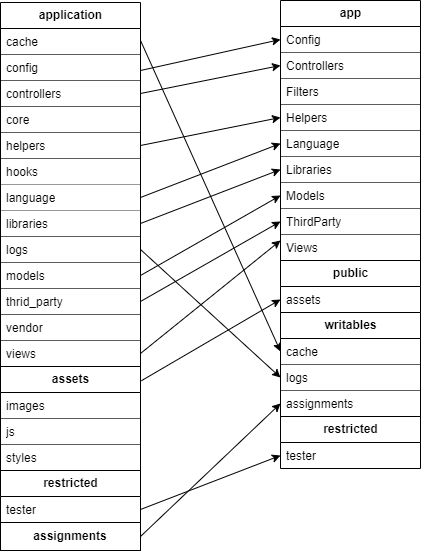
\includegraphics[scale=0.5]{dirMapping}  
	\caption[\textit{Pemindahan struktur aplikasi menuju \textit{CodeIgniter 4}}]{\textit{Pemindahan struktur aplikasi menuju \textit{CodeIgniter 4}}} 
	\label{fig:dirMapping} 
\end{figure} 

Berikut merupakan rincian direktori yang akan dipindahkan menuju \textit{CodeIgniter 4}.
\subsubsection{Application}
Direktori-direktori \texttt{application} pada \textit{CodeIgniter 3} akan dipindahkan dengan penyesuaian menuju direktori \texttt{app} terkecuali direktori \texttt{vendor}, \texttt{cache} dan \texttt{core}. Berikut merupakan direktori yang dipindahkan dari direktori \textit{application} menuju direktori \textit{app}.
\begin{itemize}
\item \verb|application/config| akan dipindahkan menuju \texttt{app/Config}.
\item \verb|application/controllers| akan dipindahkan menuju \texttt{app/Controllers}.
\item \verb|application/helpers| akan dipindahkan menuju \texttt{app/Helpers}.
\item \verb|application/languange| akan dipindahkan menuju \texttt{app/Languange}.
\item \verb|application/libraries| akan dipindahkan menuju \texttt{app/Libraries}.
\item \verb|application/models| akan dipindahkan menuju \texttt{app/Models}.
\item \verb|application/views| akan dipindahkan menuju \texttt{app/views}.
\end{itemize}

\subsubsection{\textit{Public}}
\textit{CodeIgniter 3} tidak menyediakan direktori akar berupa \textit{public} sehingga terdapat perubahan struktur dimana direktori yang sebelumnya ada pada \texttt{application} akan dipindah menuju direktori \texttt{public}. Berikut merupakan direktori yang dipindahkan menuju direktori \texttt{public}.
\begin{itemize}
\item \verb|assets| akan dipindahkan menuju \texttt{public/assets}.
\end{itemize}

Selain stuktur aplikasi diatas, \textit{SharIF Judge} memiliki dua buah direktori terpisah diluar direktori utama bernama \textit{assignments} dan \textit{tester}. Direktori \textit{assignments} ini berfungsi untuk menyimpan seluruh \textit{file} yang telah dikumpulkan sedangkan direktori \textit{tester} digunakan untuk melakukan percobaan untuk keamanan \textit{sandbox}. Kedua direktori ini harus dapat ditulis oleh \textit{PHP} sehingga akan dipindahkan menuju direktori \textit{writables}.

\subsubsection{\textit{Writables}}
Direktori ini merupakan direktori berisikan seluruh direktori yang dapat ditulis oleh \textit{PHP}. Berikut merupakan direktori yang dipindahkan menuju \textit{writables}.
\begin{itemize}
\item \verb|application/cache| akan dipindahkan menuju \texttt{writables/cache}.
\item \verb|application/log| akan dipindahkan menuju \texttt{writables/logs}.
\item \verb|assignments| akan dipindahkan menuju \texttt{writables/assignments}.
\end{itemize}

\subsection{\textit{Routing}}
\textit{Routing} pada aplikasi \textit{SharIF Judge} menggunakan \textit{auto routing} yang telah disediakan oleh \textit{CodeIgniter 3}. \textit{Auto routing} akan membentuk \textit{url} sesuai dengan \textit{controller} dan \textit{method} yang telah dibentuk tanpa harus didefinisikan secara manual. Penggunaan \textit{auto routing} seperti pada \textit{CodeIgniter 3} memiliki kekurangan pada bagian keamanan dimana \textit{filter} pada \textit{controller} dan proteksi \textit{CSRF} akan dilewati. Sehingga, konversi pada aplikasi \textit{SharIF Judge} akan menggunakan \textit{URI Routing} yang didefinisikan secara manual untuk alasan keamanan dan \textit{url} yang fleksibel. Berikut merupakan contoh \textit{route} yang didefinisikan secar a manual.
\begin{center}
\verb|$routes->post("login/register",'Login::register');|
\end{center}
\textit{Route} akan didefinisikan secara eksplisit sesuai dengan fungsinya.

\subsection{\textit{Model, View, and Controller}}
\textit{CodeIgniter 4} memiliki perubahan baik dari kegunaan dan cara pemanggilan \textit{Model, View, and Controller}. Berikut merupakan perubahan yang terjadi:
\subsubsection{\textit{Model}}
\textit{Model} pada \textit{CodeIgniter 4} memiliki perubahan dimana \textit{model} dapat digunakan untuk mengambil data pada satu buah tabel spesifik. Konversi \textit{model} dari \textit{CodeIgniter 3} menuju \textit{CodeIgniter 4} dapat dilakukan menggunakan dua buah cara yakni:
\begin{enumerate}
\item Menggunakan \textit{Model} dari \textit{CodeIgniter 3}

\textit{Model} pada \textit{CodeIgniter 3} memiliki kekurangan dimana pengguna harus membentuk secara manual seluruh fungsi untuk mengambil, memasukan, dan memperbaharui data dari sebuah tabel spesifik pada \textit{model} tersebut. Kode \ref{kode:modelCI3} merupakan contoh fungsi yang digunakan untuk mengambil data dari sebuah tabel.
\begin{lstlisting}[caption=Contoh fungsi untuk mengambil data seluruh user, label=kode:modelCI3]
public function get_all_users()
	{
		return $this->db->order_by('role', 'asc')->order_by('id')->get('users')->result_array();
	}
\end{lstlisting}

Kode \ref{kode:modelCI3} mengambil data dari tabel \texttt{users} dengan hasil berupa \textit{array} dan diurutkan sesuai dengan \texttt{role} dan \texttt{id}nya.

\item Menggunakan \textit{Model} pada \textit{CodeIgniter 4}

\textit{CodeIgnier 4} menyediakan fungsi \textit{model} yang dapat dibentuk melalui \textit{command line} untuk sebuah tabel spesifik. Pengguna dapat membentuk \textit{model} melalui \textit{command line} menggunakan sintaks sebagai berikut.
\begin{center}
	\verb|make:model <name>|
\end{center}
\textit{Model} pada \textit{CodeIgniter 4} menyediakan fungsi untuk mengambil, memasukan, dan memperbaharui data dari sebuah tabel spesifik tanpa harus membentuk secara manual fungsi-fungsi tersebut. Pengguna dapat memakai fungsi untuk mengambil data menggunakan kode berikut.
\begin{center}
	\verb|$userModel = new \App\Models\UserModel();|
\end{center}
\begin{center}
	\verb|$user = $userModel->findAll();|
\end{center}
\end{enumerate}

Kode diatas akan mengambil seluruh data dari \verb|$userModel| sesuai dengan konfigurasi yang telah dilakukan pengguna. Pengguna juga dapat melakukan \textit{create, update,} dan \textit{delete} melalui kode berikut.

\begin{lstlisting}[caption=Contoh kode untuk menghapus data pada model, label=kode:modelCI4Delete]
$this->Notifications_model->delete('notifications', array('id' => $id));

\end{lstlisting}

. Konversi aplikasi \textit{SharIF Judge} akan menggunakan kedua buah cara dengan penghapusan beberapa fungsi yang terdapat pada \textit{model} dari \textit{CodeIgniter 4} seperti mengambil, menghapus, dan menambahkan data. Sedangkan untuk fungsi-fungsi lain pada \textit{SharIF Judge} akan dilakukan pembaharuan sesuai dengan dokumentasi yang telah ada.

\subsubsection{\textit{View}}
\textit{View} pada aplikasi \textit{SharIF Judge} menggunakan \textit{template engine} bernama \textit{Twig}. \textit{Twig} merupakan sebuah \textit{template engine} untuk bahasa pemrograman \textit{PHP} yang berguna untuk mempermudah dalam mebentuk tampilan sebuah aplikasi. \textit{Twig} tidak terintegrasi pada \textit{CodeIgniter 4} sehingga akan terdapat beberapa pemasangan dan perubahan pada sintaks yang telah dipasang. Selain itu, terdapat beberapa perubahan fungsi pada \textit{CodeIgniter 4} sehingga perlu dilakukan penyesuaian seperti pengubahan \textit{file extension} dari \texttt{.twig} menjadi \texttt{.php}. Konversi \textit{SharIF Judge} menuju \textit{CodeIgniter 4} akan mengubah \textit{view} yang sebelumnya menggunakan \textit{twig} menjadi menggunakan \textit{PHP} sesuai dengan dokumentasi \textit{CodeIgniter 4}. Kode \ref{kode:viewTwig} merupakan contoh konversi yang dilakukan.

\begin{lstlisting}[caption=Contoh \textit{view} menggunakan \textit{twig}, label=kode:viewTwig]

	<a href="{{ site_url('register') }}">Register</a> |

\end{lstlisting}

menjadi kode berikut:

\begin{lstlisting}[caption=Contoh \textit{view} menggunakan \textit{php}, label=kode:viewPHP]
<?php if($registration_enabled): ?>
	<a href="<?= site_url('register') ?>">Register</a> |
<?php endif ?>
\end{lstlisting}

Seluruh sintaks \textit{twig} akan diubah menjadi sintaks \textit{PHP} dari \textit{CodeIgniter 4} seperti kode \ref{kode:viewPHP}.

\subsubsection{\textit{Controller}}
\textit{Controller} pada \textit{CodeIgniter 4} memiliki fungsi sama dengan pada \textit{CodeIgniter 3} sehingga hanya perlu dilakukan penghapusan dan perubahan pada sintaks yang ada. Namun, terdapat perubahan pada \texttt{constructor} dimana pada \textit{CodeIgniter 4} terdapat \texttt{initController}. \textit{Constructor} pada \textit{PHP} tidak diperbolehkan untuk mengembalikan apapun sehingga terdapat beberapa pemindahan fungsi seperti \texttt{redirect()} menuju \textit{filters}. Selain itu, konversi akan tetap menggunakan \verb|__construct| dengan pemindahan beberapa sintaks menuju \texttt{initController} seperti pemanggilan \textit{helpers} dan variabel yang dapat diakses pada seluruh \textit{controller}. Berikut merupakan contoh penggunaan \texttt{initController} untuk variabel.

\begin{lstlisting}[caption=Contoh penggunaan initController untuk variabel, label=kode:initController]
protected $config;

public function initController(RequestInterface $request, ResponseInterface $response, LoggerInterface $logger)
    {
        // Do Not Edit This Line
        parent::initController($request, $response, $logger);

        // Preload any models, libraries, etc, here.

        // E.g.: $this->session = \Config\Services::session();
    }
\end{lstlisting}

Kode \ref{kode:initController} akan memanggil variabel \verb|$session| yang dapat digunakan seluruh \textit{controller}.

Fungsi lainnya akan dipindahkan sesuai dengan yang ada pada \textit{CodeIgniter 3} dengan pembaharuan sesuai dengan dokumentasi \textit{CodeIgniter 4}. Selain pembaharuan, akan terdapat pemindahan variabel \textit{global} yang sebelumnya telah diinisiasikan menuju \textit{controller}.

\subsection{\textit{Libraries}}
\textit{Libraries} pada \textit{CodeIgniter 3} memiliki perubahan dan penghapusan pada \textit{CodeIgnier 4} sehingga perlu dilakukan pembaharuan. Berikut merupakan \textit{libraries} yang dipakai pada \textit{SharIF Judge}:

\subsubsection{\textit{Emails}}
\textit{Emails} pada \textit{CodeIgnier 3} terdapat perubahan sintaks dan cara pemanggilan sehingga akan dipindahkan sesuai dengan sintaks yang baru. Sintaks berubah dari yang sebelumnya menggunakan \textit{snakecase} menjadi menggunakan \textit{camelcase}. Kode \ref{} merupakan contoh penggunaan \textit{library email}.

\begin{lstlisting}[caption=Contoh penggunaan initController untuk variabel, label=kode:initController]

\end{lstlisting}

\subsubsection{\textit{Working with Uploaded Files}}
\textit{Working with uploaded files} terdapat perubahan pada beberapa sintaks dan validasi terhadap \textit{file} yang telah diunggah. Konversi aplikasi \textit{SharIF Judge} akan menggunakan fungsi ini dengan beberapa perubahan sintaks sesuai dengan dokumentasinya.

\subsubsection{\textit{Validations}}
\textit{Validations} terdapat perubahan dan pengapusan beberapa fungsi. Berikut merupakan contoh pembentukan aturan untuk mengumpulkan sebuah data pada \textit{form}.
\begin{center}
\verb|$validate->setRule('username', 'username', 'required|min\_length[3]|max\_length[20]);|
\end{center}
Sintaks diatas akan melakukan validasi terhadap \textit{input} yang akan masukan oleh pengguna. Namun, \textit{CodeIgniter 4} tidak menyediakan fungsi \texttt{form\_error} sehingga akan diubah dengan menggunakan fungsi baru bernama \texttt{validation\_errors()}. Fungsi tersebut dapat digunakan untuk mengembalikan \textit{error} apabila terdapat data yang tidak sesuai dengan aturan. \textit{Error} tersebut dapat ditampilkan pada halaman menggunakan sintaks berikut.

\begin{center}
\verb|<?php $error = $validation->getError('username'); ?>|
\end{center}

Selain menggunakan \texttt{validation\_errors()} akan digunakan sebuah fungsi \textit{flashMessage} pada \textit{session}. Fungsi ini juga dapat menampilkan \textit{error} dari data yang dimasukan pengguna apabila tidak sesuai dengan \textit{database}.

\textit{Library} yang terdapat pada \textit{CodeIgniter 4} juga dapat di\textit{extend} dan dibentuk sesuai dengan kebutuhan. Berikut merupakan \textit{library} yang dibentuk oleh pengguna. Berikut merupakan \textit{library} yang dibentuk oleh pengguna.

\subsubsection{\textit{Password\_hash}}
\textit{Library} ini dibentuk oleh \textit{phpass} untuk melakukan enkripsi \textit{password} dan melakukan verifikasi \textit{password}. \textit{Phpass} merupakan \textit{library} 

\textit{Phpass} hanya mendukung \textit{PHP} versi 5 sampai dengan 7. Sehingga, akan dilakukan konversi menggunakan fungsi yang disediakan oleh \textit{PHP} bernama \texttt{password\_hash()}. Seluruh penggunaan \textit{library} ini akan diubah menggunakan fungsi yang disediakan oleh \textit{PHP} dengan metode \textit{hashing} sama yaitu \textit{CRYPT\_BLOWFISH}.

\subsection{\textit{Configuration}}
\textit{Configuration} memiliki perubahan nama dan perpindahan beberapa sintaks. Perubahan nama terdapat pada \verb|application/config/config.php| menjadi \texttt{app/Config/App.php}. Selain itu, berikut merupakan sintaks yang dipindahkan menuju \texttt{app/Config/Security.php}:
\begin{itemize}
\item \verb|$config['csrf_protection'] = TRUE;|
\item \verb|$config['csrf_token_name'] = 'shj_csrf_token';|
\item \verb|$config['csrf_cookie_name'] = 'shjcsrftoken';|
\item \verb|$config['csrf_expire'] = 7200;|
\item \verb|$config['csrf_regenerate'] = FALSE;|
\end{itemize}

\textit{Configurations} yang telah dipindahkan akan diubah dari yang sebelumnya menggunakan \textit{array} menjadi menggunakan \textit{variable}. Seluruh \textit{configurations} pada \textit{CodeIgniter 3} akan dipindahkan menuju \textit{CodeIgniter 4} sesuai dengan direktorinya dan fungsinya.

\subsection{\textit{Database}}
\textit{Database} pada \textit{CodeIgniter 4} fungsi yang sama pada \textit{CodeIgniter 3} sehingga akan dilakukan pemindahan konfigurasi sesuai dengan yang ada pada \textit{CodeIgniter 3}. Namun, terjadi beberapa perubahan pada sintaks untuk melakukan koneksi ke \textit{database} dan beberapa sintaks untuk melakukan \textit{query}. Sintaks koneksi \textit{database} akan berubah dari \texttt{\$this->load->database();} menjadi \texttt{db = db\_connect()}. Selain itu, pemanggilan fungsi \textit{query builder} berubah menggunakan \textit{camelcase} dari yang sebelumnya menggunakan \textit{snakecase}. Seperti dari yang sebelumnya menggunakan sintaks \texttt{get\_where} menjadi \texttt{getWhere}.

\textit{Database} pada aplikasi \textit{SharIF Judge} menggunakan \textit{autoload} yang dapat memuat beberapa fungsi secara otomatis. Berikut merupakan contoh penggunakan \textit{autoload} pada \textit{CodeIgniter 3}.
\begin{center}
\verb|$autoload['libraries'] = array('database');|
\end{center}
Sintaks diatas memuat \textit{library database} dan akan  ditambahkan pada \textit{file} \texttt{autoload.php}. Namun, pada konversi ini tidak akan menggunakan \textit{autoload} karena \textit{CodeIgniter 3} tidak mengikuti standar \textit{PSR 4} sehingga pada \textit{CodeIgniter 4} akan dimuat menggunakan \texttt{db = db\_connect()} pada \texttt{initController}.

\subsection{\textit{Helpers}}
\textit{Helpers} tidak terdapat banyak perubahan namun, terdapat perubahan pemanggilan \textit{helpers} dan beberapa penghapusan \textit{helpers}. Berikut merupakan \textit{helpers} yang dihapus dan diubah cara pemanggilannya.
\begin{itemize}
\item \textit{Download Helper}
\textit{Helper} ini sudah tidak tersedia pada \textit{CodeIgniter 4} sehingga perlu dilakukan pengubahan dengan menggunakan fungsi \textit{HTTP Response}. \textit{HTTP Response} menyediakan fungsi bernama \textit{Force File Download} yang berguna untuk mengunduh sebuah \textit{file} menuju perangkat pengguna. Fungsi ini dapat dipanggil menggunakan sintaks berikut.

\begin{center}
 \verb|return $this->response->download($name, $data);|
\end{center}

Sintaks diatas mengembalikan \textit{file} yang ingin diunduh pengguna dengan dua buah parameter. Parameter pertama berupa nama \textit{file} yang ingin diunduh sedangkan parameter kedua merupakan data dalam \textit{file} tersebut.

\item \texttt{redirect()} \\
Fungsi ini memiliki perubahan pada \textit{CodeIgniter 4} dimana \texttt{redirect()} tidak langsung mengarahkan kepada \textit{url} yang dibentuk. Pengguna harus mengembalikan fungsi \textit{redirect()} menggunakan \texttt{return} dengan sintaks sebagai berikut.
\begin{center}
 \verb|return redirect()->to('login/form')|
\end{center} 

Sintaks diatas akan mengembalikan pengguna menuju \textit{url} \texttt{login/form} yang sudah dibentuk pada \textit{routes}.

\end{itemize}

Konversi \textit{helpers} akan dipindahkan dari yang sebelumnya menggunakan \textit{autoload} menuju \texttt{initController} dengan menambahkan pada variabel \textit{helpers}.

